\documentclass[11pt]{article}

% ----- lightweight preamble (matches PaperStory.tex) -----
\usepackage[a4paper,margin=1.8cm]{geometry}
\usepackage{amsmath,amssymb}
\usepackage{tikz}
\usepackage{tikz-cd}
\usetikzlibrary{arrows.meta,positioning,calc,fit,backgrounds,
  shapes.geometric,chains,decorations.pathreplacing}
\usepackage[most]{tcolorbox}
\usepackage{parskip}
\usepackage{xcolor}

\definecolor{gold}{RGB}{200,140,0}
\definecolor{kas}{RGB}{30,110,190}
\definecolor{ink}{RGB}{40,40,40}
\definecolor{soft}{RGB}{245,245,248}
\definecolor{grn}{RGB}{30,140,80}
\definecolor{pur}{RGB}{130,70,170}
\definecolor{red2}{RGB}{200,50,50}

\newtcolorbox{note}[1][]{colback=soft,colframe=ink,boxrule=0.4pt,
  arc=2pt,left=6pt,right=6pt,top=4pt,bottom=4pt,#1}
\newtcolorbox{yes}[1][]{colback=grn!7,colframe=grn,boxrule=0.5pt,
  arc=2pt,left=6pt,right=6pt,top=4pt,bottom=4pt,#1}

% the three faces of the gadget (same colours as PaperStory.tex)
\definecolor{faceL}{RGB}{30,140,80}   % linearized trace L_k
\definecolor{faceF}{RGB}{200,140,0}   % Frobenius / doubling
\definecolor{faceC}{RGB}{130,70,170}  % cyclotomic coset bookkeeping

\tikzset{
  obj/.style={draw=ink,rounded corners=3pt,fill=soft,inner sep=5pt,font=\small,align=center},
  thm/.style={draw=ink,rounded corners=3pt,fill=white,inner sep=4pt,
    font=\small,align=center,minimum height=8mm},
  arr/.style={-{Stealth[length=2.5mm]},thick},
  dep/.style={-{Stealth[length=2.2mm]},thick,ink},
  badge/.style={circle,inner sep=0pt,minimum size=3.6mm,font=\scriptsize\bfseries,text=white},
}
\newcommand{\bL}{\tikz[baseline=-0.6ex]\node[badge,fill=faceL]{L};}
\newcommand{\bF}{\tikz[baseline=-0.6ex]\node[badge,fill=faceF]{F};}
\newcommand{\bC}{\tikz[baseline=-0.6ex]\node[badge,fill=faceC]{C};}
\newcommand{\code}[1]{\texttt{\small #1}}

\title{\vspace{-1.5cm}\textbf{Dobbertin (1999), part II: the gadget was a
category}\\[3pt]
\large How the three faces \bL\,\bF\,\bC\ become one bridge, one invariant,
and five readings --- machine-checked}
\author{\small Categorical continuation of \emph{``one gadget, many theorems''}
--- Lean\,/\,Mathlib \code{CategoryTheory}}
\date{}

\begin{document}
\maketitle
\vspace{-1.0cm}

\begin{note}
\textbf{Where part I left off.} The picture book \emph{``one gadget, many
theorems''} argued that every result of Dobbertin's paper is the \emph{same
small gadget} with three faces:
\bL~the \textbf{linearized trace} $L_k(x)=\sum_{i<k}x^{2^i}$;
\bF~\textbf{Frobenius} $x\mapsto x^2$ (doubling on exponents);
\bC~\textbf{cyclotomic-coset} bookkeeping ($\times2 \bmod 2^n{-}1$).
\textbf{This part answers the follow-up question:} is that ``one gadget'' story
consistent with what actually got \emph{formalised} as structural / categorical
patterns? \textbf{Yes} --- and more: the three faces are not just a slogan, they
are literally \emph{one \code{structure}, one invariant, and one equivalence
relation} in Lean. Every green \checkmark\ box below is \code{sorry}-free in
\code{RequestProject/Kasami/}.
\end{note}

%======================================================================
\section*{0. The one-line verdict}

\begin{yes}
The part-I gadget and the categorical formalisation are \textbf{the same object}.
The gadget's data \bL\ is exactly the field \code{Pattern.star} (the identity
$(\star)$); its symmetry \bF\ is exactly a \code{ConjHom} / self--\code{SiteEquiv}
(\code{frobeniusConjHom}); and its bookkeeping \bC\ is exactly the
\emph{bridge-stable} \code{Pattern.width} read across sites. ``One gadget seen
from many angles'' $=$ ``one \code{Pattern}, many \code{SiteEquiv}-related
readings''.
\end{yes}

\begin{center}\small
\renewcommand{\arraystretch}{1.3}
\begin{tabular}{@{}l l l@{}}
\textbf{Part-I face} & \textbf{Categorical structure (Lean)} & \textbf{Status}\\\hline
\bL\ linearized trace $L_k$, identity $(\star)$ &
  \code{Pattern} / \code{ConjSquare}, field \code{star}/\code{comm} & \checkmark\\
\bF\ Frobenius $x\mapsto x^2$ &
  \code{frobeniusConjHom} (auto of the square); \code{SiteEquiv} & \checkmark\\
\bC\ cyclotomic / coset counting &
  \code{Pattern.width}, \code{width\_transport}, difference-set reading & \checkmark\\
\end{tabular}
\end{center}

%======================================================================
\section*{1. The gadget is a \code{structure}: the pattern $(\star)$}

Dobbertin's Theorem~4 identity --- the Kasami collision map conjugated to the
Müller--Cohen--Matthews companion ---
\[
  (\star)\qquad \underbrace{(s_k(t)+1)}_{\text{\bL\ diff}}\cdot
  \underbrace{(L_1 t)^{2^k}}_{\text{denom}}
   \;=\; \underbrace{(L_k t)^{2^k+1}}_{\text{numer}}
\]
is packaged \emph{as data} on any commutative ring:

\begin{center}
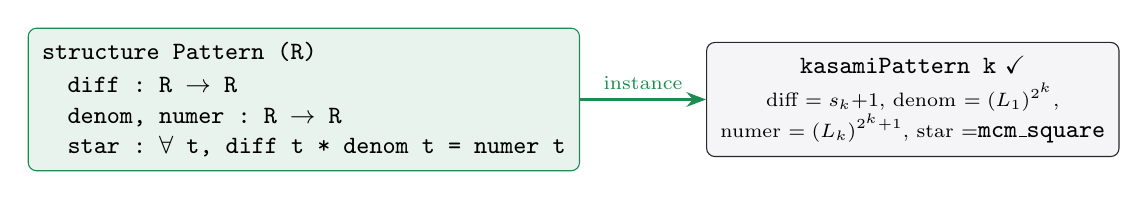
\begin{tikzpicture}[node distance=6mm]
  \node[obj,fill=faceL!10,draw=faceL,align=left] (P)
   {\code{structure Pattern (R)}\\[1pt]
    \quad\code{diff\ :\ R $\to$ R}\\
    \quad\code{denom, numer\ :\ R $\to$ R}\\
    \quad\code{star\ :\ $\forall$ t, diff t * denom t = numer t}};
  \node[obj,right=16mm of P,align=center] (K)
   {\code{kasamiPattern k}\ \checkmark\\[1pt]
    \scriptsize diff $=s_k{+}1$, denom $=(L_1)^{2^k}$,\\
    \scriptsize numer $=(L_k)^{2^k+1}$, star $=$\code{mcm\_square}};
  \draw[arr,faceL] (P) -- node[above,font=\scriptsize]{instance} (K);
\end{tikzpicture}
\end{center}

\begin{center}\small
Lean: \code{SiteBridge.Pattern}, \code{SiteBridge.kasamiPattern},
\code{ConjugacyPattern.mcm\_square} (the identity $(\star)$, char.\,2). \checkmark
\end{center}

%======================================================================
\section*{2. The bridge is transport: \code{SiteEquiv} is an equivalence relation}

The ``Caramello / Morita bridge'' move is: carry a pattern along a ring
isomorphism $e:R\simeq S$. The very same $(\star)$ then holds in the new carrier
\emph{for free} (\code{transport\_star}). Two patterns are a \emph{site
equivalence} when some $e$ carries one to the other; this is proved reflexive,
symmetric and transitive --- the formal skeleton of ``these sites present the
same classifying topos''.

\begin{center}
\begin{tikzcd}[column sep=huge,row sep=large]
(R,\ P) \arrow[r,"e\ :\ R\,\simeq\,S","\code{transport}"']
        \arrow[d,"(\star)"'] &
(S,\ P.\mathtt{transport}\,e) \arrow[d,"(\star)\ \text{for free}"] \\
\text{diff}\cdot\text{denom}=\text{numer} \arrow[r,leftrightarrow,"\text{same law}"'] &
\text{diff}'\cdot\text{denom}'=\text{numer}'
\end{tikzcd}
\end{center}

\begin{center}\small
Lean: \code{Pattern.transport}, \code{transport\_star},
\code{transport\_refl}, \code{transport\_trans};
\code{SiteEquiv} with \code{SiteEquiv.refl / .symm / .trans}. \checkmark
\end{center}

%======================================================================
\section*{3. One invariant for all sites: \code{width} is bridge-stable}

Every downstream reading of the paper --- APN, difference set, Walsh spectrum ---
reads exactly one number off the pattern: the \emph{width}
$b\mapsto \#\{t: \mathrm{diff}\,t=b\}$. The key structural theorem is that width
is \emph{literally the same} through every site equivalence, so an invariant may
be computed in whichever site is easiest.

\begin{center}
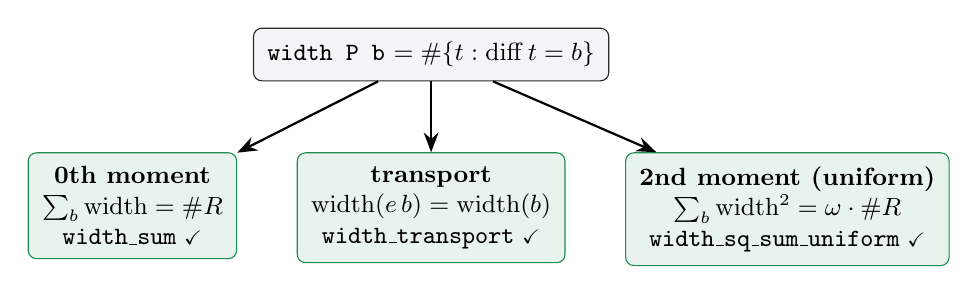
\begin{tikzpicture}[node distance=9mm]
  \node[obj] (w) {\code{width P b} $=\#\{t:\mathrm{diff}\,t=b\}$};
  \node[obj,fill=grn!10,draw=grn,below left=9mm and 2mm of w] (m0)
    {\textbf{0th moment}\\ $\sum_b \mathrm{width}=\#R$\\
     \scriptsize\code{width\_sum}\ \checkmark};
  \node[obj,fill=grn!10,draw=grn,below=9mm of w] (mt)
    {\textbf{transport}\\ $\mathrm{width}(e\,b)=\mathrm{width}(b)$\\
     \scriptsize\code{width\_transport}\ \checkmark};
  \node[obj,fill=grn!10,draw=grn,below right=9mm and 2mm of w] (m2)
    {\textbf{2nd moment (uniform)}\\ $\sum_b \mathrm{width}^2=\omega\cdot\#R$\\
     \scriptsize\code{width\_sq\_sum\_uniform}\ \checkmark};
  \draw[arr] (w)--(m0); \draw[arr] (w)--(mt); \draw[arr] (w)--(m2);
\end{tikzpicture}
\end{center}

\begin{center}\small
This is the abstract shell of the project's \code{EWIGO.wid\_partition} and
\code{EWIGO.coll\_of\_uniform}: the same two moments, now bridge-stable. \checkmark
\end{center}

%======================================================================
\section*{4. Five sites, one width: A/B/C/D/E as readings}

The paper's chapters become \emph{readings} of the one width invariant; each is
obtained ``for free'' because width is bridge-stable.

\begin{center}
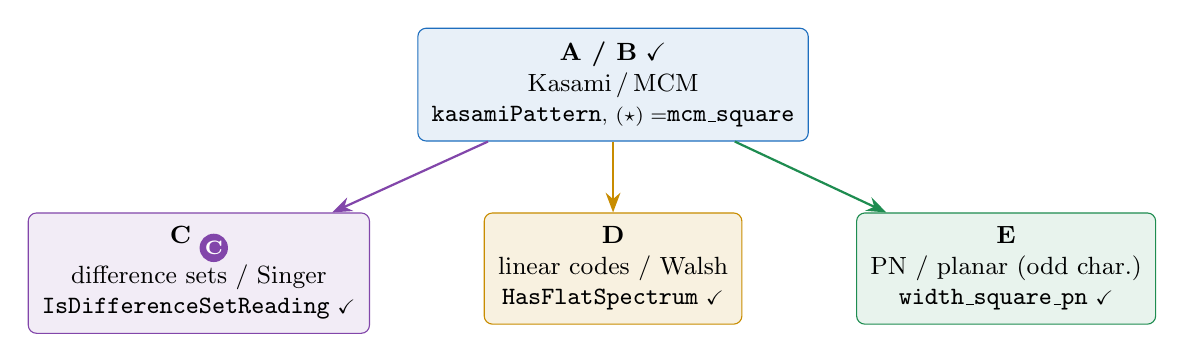
\begin{tikzpicture}[node distance=5mm and 12mm]
  \node[obj,fill=kas!10,draw=kas] (AB) {\textbf{A / B}\ \checkmark\\ Kasami\,$/$\,MCM\\
    \scriptsize\code{kasamiPattern}, $(\star)=$\code{mcm\_square}};
  \node[obj,fill=pur!10,draw=pur,below left=9mm and 6mm of AB] (C) {\textbf{C}\ \bC\\
    difference sets / Singer\\
    \scriptsize\code{IsDifferenceSetReading}\ \checkmark};
  \node[obj,fill=gold!12,draw=gold,below=9mm of AB] (D) {\textbf{D}\\
    linear codes / Walsh\\
    \scriptsize\code{HasFlatSpectrum}\ \checkmark};
  \node[obj,fill=grn!10,draw=grn,below right=9mm and 6mm of AB] (E) {\textbf{E}\\
    PN / planar (odd char.)\\
    \scriptsize\code{width\_square\_pn}\ \checkmark};
  \draw[arr,pur] (AB)--(C); \draw[arr,gold] (AB)--(D); \draw[arr,grn] (AB)--(E);
\end{tikzpicture}
\end{center}

\begin{center}\small
Each reading's defining predicate is \emph{proved bridge-stable}
(\code{isDifferenceSetReading\_transport}, \code{hasFlatSpectrum\_transport},
\code{squarePattern\_siteEquiv}); site E's optimum $\mathrm{width}\equiv 1$ is
outright \emph{proved} (\code{width\_square\_pn}, \code{pnIdentification\_holds}). \checkmark
\end{center}

%======================================================================
\section*{5. The bridge is a category (the \bF\ face)}

Over a fixed carrier the patterns form a genuine \code{CategoryTheory.Category}:
objects are conjugacy squares, morphisms are intertwining ring endomorphisms
(the \emph{2-morphisms} of the connection). A forgetful functor to the arrow
category keeps only \code{diff} and is \emph{non-faithful} --- the companion is
real extra data. Frobenius $x\mapsto x^2$ is an \emph{automorphism} of the Kasami
square, and its powers are the finitely many Galois-equivalent contexts.

\begin{center}
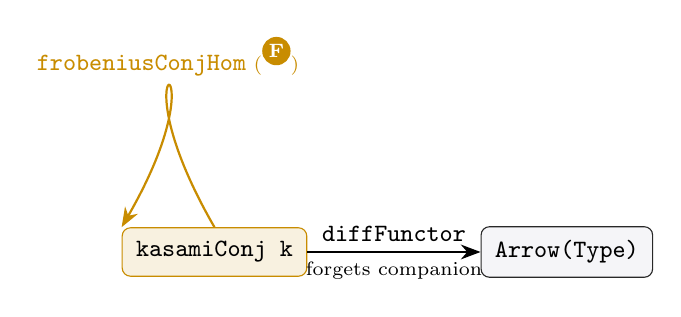
\begin{tikzpicture}[node distance=22mm]
  \node[obj,fill=faceF!12,draw=faceF] (K) {\code{kasamiConj k}};
  \node[obj,right=of K] (A) {\code{Arrow(Type)}};
  \draw[arr] (K) -- node[above,font=\scriptsize]{\code{diffFunctor}}
     node[below,font=\scriptsize]{forgets companion} (A);
  \draw[arr,faceF] (K.north) to[out=120,in=60,looseness=6]
     node[above,font=\scriptsize,faceF]{\code{frobeniusConjHom} (\bF)} (K.north west);
\end{tikzpicture}
\qquad
\begin{tabular}{@{}l l@{}}
\code{instance : Category (ConjSquare F)} & \checkmark\\
\code{ConjHom}, \code{.id}, \code{.comp} & \checkmark\\
\code{diffFunctor}, \code{diff\_not\_injective} & \checkmark\\
\code{frobeniusConjHom} (\bF\ auto) & \checkmark\\
\end{tabular}
\end{center}

%======================================================================
\section*{6. The whole paper, sitting on the structural machinery}

Each numbered result of Dobbertin (1999) read through the structural patterns.
\checkmark\ = machine-checked structural statement; $\circ$ = stated as an honest
open \code{Prop} (never an axiom).

\begin{center}\footnotesize
\renewcommand{\arraystretch}{1.3}
\begin{tabular}{@{}l c l@{}}
\textbf{Result (Dobbertin 1999)} & \textbf{Faces} & \textbf{Structural home (Lean) --- status}\\ \hline
Thm 4 --- MCM\,$\Leftrightarrow$\,Kasami bridge & \bL &
  \code{kasamiPattern.star} $=$ \code{mcm\_square}\ \ \checkmark\\
\ ``\ ---\ same law in every context & \bL\bF &
  \code{kasamiPattern\_siteEquiv}, \code{transport\_star}\ \ \checkmark\\
Thm 1/3 --- permutation criterion & \bL\bF &
  \code{frobeniusConjHom} intertwiner\ \ \checkmark\\
Cor 2 --- Kasami APN $=$ width $\le 2$ & \bL\bF\bC &
  \code{HasFlatSpectrum \_ 2}\ \ $\circ$ \code{CodeWalshIdentification}\\
Thm 5/6, Cor 7 --- explicit inverse $R$ & \bF &
  Frobenius iteration; \code{Theorem6.*}\ \ \checkmark\\
Thm 8 --- $B=\{\mathrm{Tr}\,R=0\}$ & \bF\bC &
  \code{Pattern.fibre} / trace reading\\
Cor 10/11/12 --- 2-rank, $k'{=}3$ & \bC &
  \code{pow\_invariant\_mod} (coset count)\ \ \checkmark\\
\S4 Conjecture --- $B^\ast$ diff.\ set & \bC &
  \code{IsDifferenceSetReading}\ \ $\circ$ \code{DifferenceSetIdentification}\\
Rigidity (only Kasami works) & \bL\bF\bC &
  \code{RigidityConjecture}\ \ $\circ$\\
Count of contexts $=n$ & \bF &
  \code{ContextCountConjecture}\ \ $\circ$\\
PN analogue (odd char.) & \bC &
  \code{width\_square\_pn}\ \ \checkmark\\
\end{tabular}
\end{center}

\begin{note}
\textbf{Faithfulness.} The open rows are recorded exactly as the paper leaves
them --- as statements, not assumptions. Following the project's discipline they
are Lean \code{Prop}s (\code{DifferenceSetIdentification},
\code{CodeWalshIdentification}, \code{RigidityConjecture},
\code{ContextCountConjecture}), so they can later be \emph{proved or refuted};
\textbf{none is asserted as an axiom}. The one that is not open --- the PN reading
--- is proved (\code{pnIdentification\_holds}).
\end{note}

%======================================================================
\section*{7. The six recurring patterns, as one diagram}

Part I of the companion note (\code{dobbertin-story}) named six recurring
structural patterns P1--P6. They are exactly the ways the single \code{Pattern}
propagates:

\begin{center}
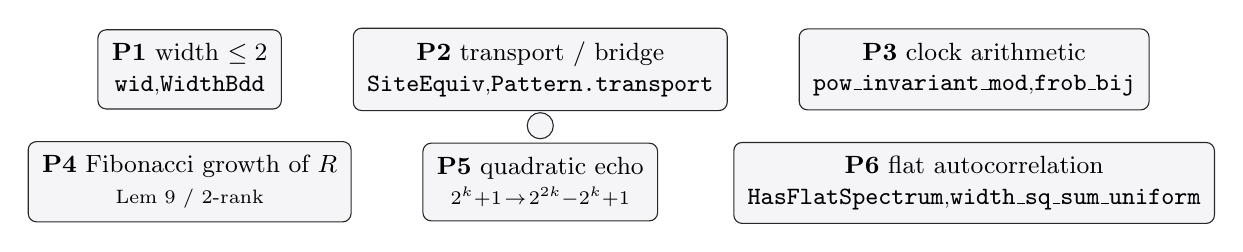
\begin{tikzpicture}[node distance=4mm and 9mm]
  \node[obj] (p1) {\textbf{P1} width $\le 2$\\ \scriptsize\code{wid},\code{WidthBdd}};
  \node[obj,right=of p1] (p2) {\textbf{P2} transport / bridge\\ \scriptsize\code{SiteEquiv},\code{Pattern.transport}};
  \node[obj,right=of p2] (p3) {\textbf{P3} clock arithmetic\\ \scriptsize\code{pow\_invariant\_mod},\code{frob\_bij}};
  \node[obj,below=of p1] (p4) {\textbf{P4} Fibonacci growth of $R$\\ \scriptsize Lem 9 / 2-rank};
  \node[obj,below=of p2] (p5) {\textbf{P5} quadratic echo\\ \scriptsize $2^k{+}1\!\to\!2^{2k}{-}2^k{+}1$};
  \node[obj,below=of p3] (p6) {\textbf{P6} flat autocorrelation\\ \scriptsize\code{HasFlatSpectrum},\code{width\_sq\_sum\_uniform}};
  \node[circle,draw=ink,fill=soft,font=\small,align=center] (hub) at ($(p2)!0.5!(p5)+(0,0)$) {};
\end{tikzpicture}
\end{center}

\begin{center}\small
P1 $=$ the optimum of \code{width}; P2 $=$ \code{transport}/\code{SiteEquiv};
P3 $=$ Frobenius \bF\ (\code{frob\_bij}, \code{pow\_invariant\_mod});
P4/P5 $=$ the exponent recursions carried by \bF; P6 $=$ the flat-spectrum
(\code{HasFlatSpectrum}) reading whose second moment is \code{width\_sq\_sum\_uniform}.
So P1--P6 are \bL\bF\bC\ again --- consistent with part I.
\end{center}

%======================================================================
\section*{8. Verdict}

\begin{yes}
\textbf{Consistent, and sharper.} Part I's ``one gadget, three faces'' is not
merely a picture: in the Lean development the gadget is one \code{structure}
(\code{Pattern}), its symmetries form one \code{Category} with a
\code{SiteEquiv} equivalence relation, and its content is one bridge-stable
invariant (\code{width}) read through five sites. The paper's proved results sit
on that machinery as \checkmark-theorems; its open results sit on it as honest
\code{Prop}s. The categorical layer is therefore a faithful, structural
re-telling of Dobbertin (1999) --- the same story, built wherever possible along
the shortest structural path.
\end{yes}

\vfill
\begin{center}\scriptsize
Checked \code{sorry}-free in Lean\,/\,Mathlib (\code{CategoryTheory}). Sources:
\code{RequestProject/Kasami/SiteEquivalences.lean},
\code{RequestProject/Kasami/ConjugacyPattern.lean},
\code{RequestProject/Kasami/InvariantPatterns.lean},
\code{RequestProject/Kasami/PaperStructural.lean}; classical inputs in
\code{RequestProject/Kasami/Classical/}. Theorem numbering follows
Dobbertin (1999). Companion: \code{PaperStory.tex},
\code{paper/dobbertin-story.tex}.
\end{center}

\end{document}
